% VUT FIT MITAI
% MSZ 2021/2022
% Author: Vladimir Dusek
% Login: xdusek27

%%%%%%%%%%%%%%%%%%%%%%%%%%%%%%%%%%%%%%%%%%%%%%%%%%%%%%%%%%%%%%%%%%%%%%%%%%%%%%%%

% Path to figures
\graphicspath{{kry/sprava_klicu_v_asymetricke}}

%%%%%%%%%%%%%%%%%%%%%%%%%%%%%%%%%%%%%%%%%%%%%%%%%%%%%%%%%%%%%%%%%%%%%%%%%%%%%%%%

\chapter{KRY -- Správa klíčů v~asymetrické kryptografii (certifikáty X.509).}

%%%%%%%%%%%%%%%%%%%%%%%%%%%%%%%%%%%%%%%%%%%%%%%%%%%%%%%%%%%%%%%%%%%%%%%%%%%%%%%%

\section{Metadata}

\begin{compactitem}
    \item Předmět: Kryptografie (KRY)
    \item Přednáška:
    \begin{compactitem}
        \item \path{KRY04_Asym_MNG.pdf}
    \end{compactitem}
    \item Záznam:
    \begin{compactitem}
        \item 2021-03-29
    \end{compactitem}
\end{compactitem}

%%%%%%%%%%%%%%%%%%%%%%%%%%%%%%%%%%%%%%%%%%%%%%%%%%%%%%%%%%%%%%%%%%%%%%%%%%%%%%%%

\section{Úvod a kontext}

\textit{Viz. \uv{Úvod a kontext} v~předchozích otázkách z~tohoto předmětu.}

\paragraph*{Problém se zveřejňováním veřejných klíčů} Jak můžu vědět, že publikovaný veřejný klíč patří opravdu entitě, které patřit má? Je potřeba zajistit autenticitu (pravost) veřejných klíčů~--~Vytvořit spolehlivou vazbu mezi veřejným klíčem a jménem jeho vlastníka.

\paragraph*{Systémy založené na veřejném klíči} Systémy založené na veřejném klíči (PKI, \textit{Public Key Infrastructure}) je označení infrastruktury správy a distribuce veřejných klíčů. PKI umožňuje pomocí přenosu důvěry používat cizí veřejné klíče a ověřovat jimi elektronické podpisy bez nutnosti jejich individuální kontroly.

%%%%%%%%%%%%%%%%%%%%%%%%%%%%%%%%%%%%%%%%%%%%%%%%%%%%%%%%%%%%%%%%%%%%%%%%%%%%%%%%

\section{Správa klíčů v~asymetrické kryptografii}

\paragraph*{Certifikát} Certifikace veřejného klíče. Nějaký prostředník (certifikační autorita), kterému důvěřujeme, se zaručuje, že konkrétní veřejný klíč, patří dané entitě.

\paragraph*{Certifikační autorita} Certifikační autorita (CA) je prostředník, který distribuuje certifikáty a které všichni důvěřují. CA negeneruje klíče uživatelům, ty si je generují samy.

\paragraph*{Proces certifikace klíče} CA podepíše veřejný klíč uživatele a jeho další údaje (jméno, doba vydání, doba platnosti, \dots) svým soukromým klíčem. Tyto podepsané údaje se nazývají certifikát.

\begin{figure}[H]
    \centering
    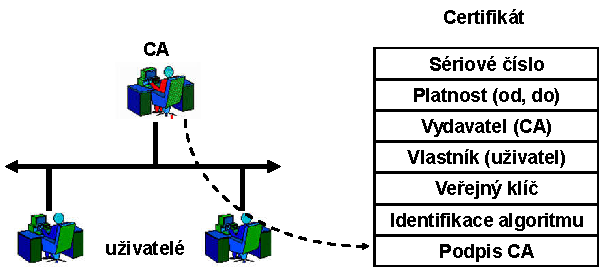
\includegraphics[width=0.65\linewidth]{certifikat.pdf}
    \caption{Příklad certifikátu.}
\end{figure}

\begin{figure}[H]
    \centering
    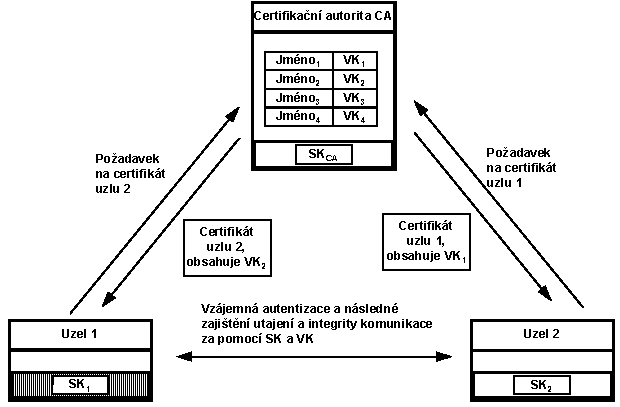
\includegraphics[width=1\linewidth]{vymena_certifikatu.pdf}
    \caption{Příklad navázání bezpečné komunikace mezi dvěma entitami, které mají stejnou certifikační autoritu.}
    \label{53_vymena_certifikatu}
\end{figure}

\paragraph*{Navázání bezpečné komunikace} Popis navázání bezpečné komunikace (viz obrázek~\ref{53_vymena_certifikatu}):
\begin{compactenum}
    \item Uzel 1 si vygeneruje soukromý a veřejný klíč.

    \item Uzel 1 odešle veřejný klíč certifikační autoritě spolu se svým jménem (a dalšíma informacema).

    \item CA vytvoří certifikát pro uzel 1~--~svým soukromým klíčem podepíše veřejný klíč a jméno uzlu 1. CA odešle certifikát uzlu 1. CA odešle svůj veřejný klíč uzlu 1.

    \item Pokud uzel 2 chce také odesílat, provede také kroky 1-3.

    \item Uzel 1 podepíše soubor a odešle ho uzlu 2 (soubor a podpis).

    \item Uzel 2 si musí sehnat certifikát uzlu 1. Existují 3 způsoby jak to udělat. \begin{compactitem}
        \item Odesílatel zašle svůj certifikát společně se zprávou.
        \item Příjemce si vyžádá certifikát odesílatele od certifikační autority.
        \item Příjemce si vyžádá certifikát odesílatele od jiné služby (adresářové služby, LDAP).
    \end{compactitem}

    \item Uzel 2 ověří podpis u~certifikátu uzlu 1 veřejným klíčem certifikační autority.

    \item Uzel 2 ověří podpis souboru pomocí veřejného klíče odesílatele (který je v~certifikátu).
\end{compactenum}

\paragraph*{Strom certifikačních autorit} Model s~jednou globální CA je nemožný (příliš mnoho uživatelů, přiliš velké vzdálosti, \dots). Proto se používá strom certifikačních autorit. Veřejný klíč CA je certifikován jinou CA. CA nejvýše ve stromu se nazývá \textbf{kořenová certifikační autorita}. \begin{compactitem}
    \item Certifikační autorita má svůj vlastní certifikát, který je podepsaný její certifikační autoritou.
    \item Koncový uživatel důvěřuje stále pouze jedné entitě~--~kořenové certifikační autoritě, ale přibývá jedna úroveň ověřování navíc.
    \item Příjemce dostane zprávu s~podpisem. Musí znát certifikát odesílatele (podepsaný $CA$), certifikát certifikační autority (podepsaný $CA_{root}$) a veřejný klíč kořenové CA\footnote{Veřejný klíč kořenové certifikační autority se z~praktických distribuuje ve formě \uv{fiktivního certifikátu}}.
    \item Úrovní certifikačních autorit může být více (nejčastěji 1-2).
\end{compactitem}

\begin{figure}[H]
    \centering
    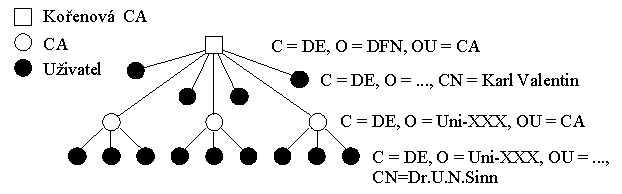
\includegraphics[width=1\linewidth]{certifikacni_strom.pdf}
    \caption{Příklad stromu certifikačních autorit. C, O, OU je identifikátor entity.}
\end{figure}

\paragraph*{Certifikační cesta} Posloupnost certifikátů od certifikátu kořenové CA přes certifikáty dalších CA až k~certifikátu komunikující protistrany.

\paragraph*{Zneplatnění certifikátu} Jak zrušit platnost certifikátu? Normálně se zruší sám, až skončí jeho platnost. Pokud je potřeba certifikát zneplatnit před jeho vypršením je třeba využít tzv. revokační seznam (CRL, \textit{certificate revocation list}). Důvody zneplatnění certifikátu: \begin{compactitem}
    \item soukromý klíč uživatele byl kompromitován,
    \item uživatel ztratil práva, která z~certifikátu vyplývají (např. změna zaměstnavatele),
    \item soukromý klíč CA byl kompromitován (nikdy se nestalo).
\end{compactitem}

\paragraph*{CRL} CRL (\textit{certificate revocation list}) je seznam zneplatněných certifikátů, takových, kterým ještě nevypršela platnost, ale je třeba je zneplatnit. CRL je podepsán CA, které ho spravuje a periodicky aktualizuje (může se zkracovat i růst). Jak se distribuuje:\begin{compactitem}
    \item \textit{Pull model}~--~Příjemce certifikátu si dle potřeby stáhne CRL od CA.
    \item \textit{Push model}~--~CA pravidelně posílá CRL příjemcům certifikátu.
\end{compactitem}

\paragraph*{Křížový certifikát} V~případě, že spolu komunikují uživatelé, kteří nemají společnou kořenovou CA (jejich CA si nedůvěřují), je třeba využít tzv. křížový certifikát. Tím se komplikuje sestavování certifikační cesty, protože je třeba zvážit všechny křížové certifikáty, které jsou k~dispozici.

\begin{figure}[H]
    \centering
    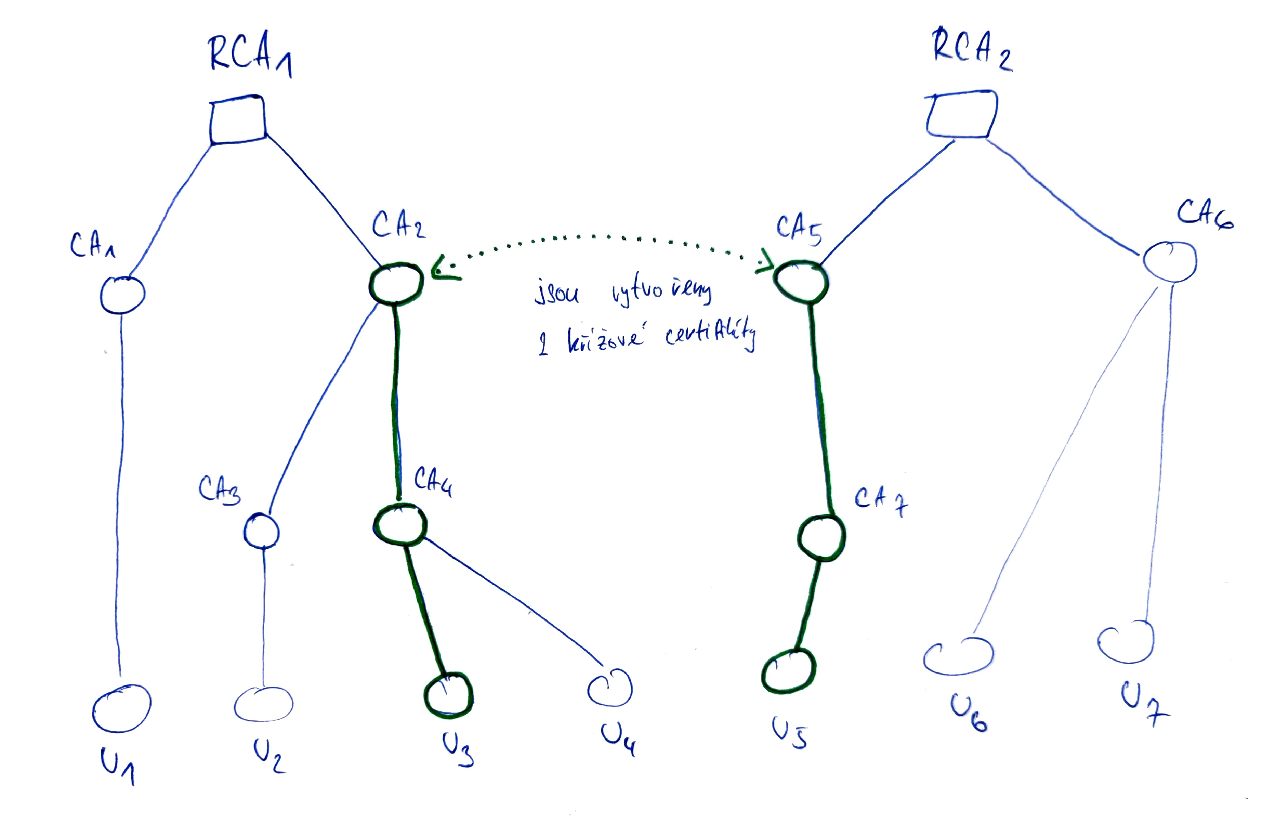
\includegraphics[width=1\linewidth]{krizovy_certifikat.pdf}
    \caption{Příklad křížového certifikátu. Uživatel $U_3$ chce navázat bezpečné spojení s~uživatelem $U_5$. Nemají společnou kořenovou CA, proto je třeba využít křížové certifikáty. CA2 vytvoří křížový certifikát pro $CA_5$ a $CA_5$ vytvoří křížový certifikát pro $CA_2$. Příklad: $U_3$ pošle podepsanou zprávu $U_5$, jak bude vypadat certifikační cesta? $U_3 \leftarrow CA_4 \leftarrow CA_2 \leftarrow CA_5 \leftarrow RCA_2$.}
\end{figure}

%%%%%%%%%%%%%%%%%%%%%%%%%%%%%%%%%%%%%%%%%%%%%%%%%%%%%%%%%%%%%%%%%%%%%%%%%%%%%%%%

\section{Standard X.509}

X.509 je standard pro systémy založené na veřejném klíči (PKI). Specifikuje formát certifikátů, formát CRL, parametry certifikátů, metody kontroly platností certifikátů, \dots

\bigskip\noindent\begin{minipage}{\linewidth}
\begin{lstlisting}[language=Python, caption={Příklad definice certifikátu ve formátu X.509.}]
Certificate ::= SIGNED SEQUENCE {
    version [0] Version DEFAULT v1988,
    serialNumber CertificateSerialNumber,
    signature
    AlgorithmIdentifier,
    issuer
    Name,
    validity
    Validity,
    subject
    Name,
    subjectPublicKeyInfo SubjectPublicKeyInfo
}

Version ::= INTEGER { v1988(0) }

CertificateSerialNumber ::= INTEGER

Validity ::= SEQUENCE { notBefore UTCTime, notAfter UTCTime }

SubjectPublicKeyInfo ::= SEQUENCE {
    algorithm
    AlgorithmIdentifier,
    subjectPublicKey
    BIT STRING
}

AlgorithmIdentifier ::= SEQUENCE {
    algorithm
    OBJECT IDENTIFIER,
    parameters
    ANY DEFINED BY algorithm OPTIONAL
}
\end{lstlisting}
\end{minipage}

\paragraph*{Význam položek} Význam položek v~definici certifikátu ve formátu X.509: \begin{compactitem}
    \item Version -- Standardně 0.
    \item Serial number -- Sériové číslo certifikátu, spolu se jménem vydavatele jednoznačně identifikuje certifikát.
    \item Issuer -- Jméno vydávající CA.
    \item Subject -- Jméno vlastníka certifikátu.
    \item Validity -- Doba platnosti certifikátu (\path{notBefore}, \path{notAfter}). Podpis je platný pouze pokud je datum podepsání v~intervalu platnosti každého z~certifikátů z~certifikační cesty.
    \item SubjectPublicKeyInfo -- Veřejný klíč vlastníka certifikátu a algoritmus, pro který je určen.
    \item Signature -- Jakým algoritmem je certifikát podepsaný CA.
\end{compactitem}

\paragraph*{Prototypový certifikát} Má strukturu certifikátu X.509. Uživatel si vygeneruje tzv. prototypový certifikát, který má standardní strukturu a vyplní informace na nějaké implicitní hodnoty. Prototyp pošle CA spolu se svým veřejným klíčem, která certifikát dovyplní, podepíše a pošle zpět.

\paragraph*{Registrační autorita} Pokud chce uživatel vydat certifikát, kontaktuje tzv. registrační autoritu (nikoliv přímo CA).

\paragraph*{Míra důvery v~certifikát}  V~praxi chceme více urovní důvěry, než pouze ostrý/žádný (např. chceme vytvořit testovací certifikát). To je řešeno jako rozšíření X.509 přidáním třídy certifikátu (\textit{certification class}). Uživatel chce vydat certifikát od CA jisté třídy. \begin{compactitem}
    \item Třída 1~--~CA vůbec nekontroluje identitu žadatele. Lze jej získat anonymně. Používá se pro testovací certifikáty.
    \item Třída 2~--~Identita žadatele musí být ověřena třetí stranou (notářsky ověřený formulář zaslaný poštou).
    \item Třída 3~--~Standardní certifikát. Žadatel musí osobně navštívit CA (resp. registrační autoritu). Osobní ověření totožnosti.
    \item Třída 4~--~Stejné jako 3 a navíc je nutné prokázat oprávnění žadatele požadovat certifikát.
\end{compactitem}

\begin{figure}[H]
    \centering
    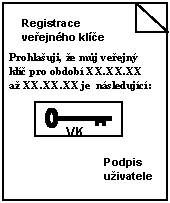
\includegraphics[width=0.35\linewidth]{registrace_certifikatu.pdf}
    \caption{Příklad žádosti o~certifikát.}
\end{figure}
